% !Mode:: "TeX:UTF-8"
% !TEX root = ..\thesis.tex
\chapter{计算实验及算法评估}
本章将对上一章的算法进行评估,通过设计相关计算实验,建立评价体系,具体评估各算法的效果及其适用规模。然后根据实验结果,为研究对象制定合适的调度方案。

\section{实验设计}
实验设计分为两个主要部分,一个是装配生产信息的生成,包括订单数量、流水线数量、各订单切换准备时间、个订单进入系统时间及其所含作业的信息;另一个是相关参数的确定,包括迭代次数、禁忌列表长度的等。
\subsection{生产装配信息生成}
生产装配信息皆由随机数产生,主要包括订单及其作业的数量信息、时间信息及惩罚系数,需要给出适当的取值范围及分布。
\begin{asparaenum}
\item 数量信息
\suspend{asparaenum}

由\reft{tab:2jobshopinfo},设计实验中的流水线的数量$m$分别为$5,6,7$,订单品种数量的范围是$[29,777]$,据此可以设计合理的订单数量$n$分别为$20,30,50,70,100,150,200,300,500,750,1000$,再根据大批量的特点,可以设置订单中作业的批量范围为$(1000,2000)$。
\resume{asparaenum}
\item 时间信息
\suspend{asparaenum}

出于保护该公司的生产能力数据,实验中所采用的时间单位是经变换过的$tu$,由于每个订单的作业批量都比较大,所以订单中的作业处理时间单位为$1/500\ tu$。订单中的作业处理时间服从参数$\alpha = 5$的负指数分布,订单到达系统的时间间隔服从参数$\lambda = 3$的泊松分布
\resume{asparaenum}
\item 惩罚系数与优先系数
\end{asparaenum}

多品种多装配线轮番装配调度优化模型的目标函数\eqref{equ:objmain}中,延迟完成的订单有惩罚系数$wt$,订单的完成有优先系数$wc$,考虑插单的模型也有类似的这两类系数,皆由随机数产生。与模型中不同的是,由于订单中的批量增多,这些系数若满足求和为$1$的约束使得每个系数的值都很小,不利计算的准确性,而同时成倍扩大不影响调度的结果,所以这些系数不作求和为$1$的处理。

实验信息数据生成的代码见附录(experiment\_data.py),生成的数据在目录(.\textbackslash data\textbackslash)中,举例来说,$20$件订单的数据所含内容\footnote{本课题提出的两个模型使用相同的数据,考虑插单的模型将用到进入系统时间$r_j$}如\reft{tab:20itemsdata}所示。
\begin{table}[h]
  \centering
  \caption{$20$件订单的实验信息数据}
    \begin{tabular}{ccccccc}
     	&	&	&	&	&	&\multicolumn{1}{r}{单位:$tu$}\\
    \toprule
    订单序号 & 装配时间 & 进入系统时刻 & 切换准备时间& 约定工期 & 主要目标权重 & 次要目标权重 \\
    ($j$) & ($p_j$) & ($r_j$) &($s_j$) &($d_j$) &($w_{(t)}$) & ($w_c$) \\
    \midrule
    1     & 23    & 56    & 7     & 100   & 15    & 2 \\
    2     & 40    & 30    & 1     & 116   & 8     & 3 \\
    3     & 36    & 20    & 7     & 98    & 10    & 4 \\
    4     & 25    & 4     & 2     & 49    & 12    & 10 \\
    5     & 17    & 5     & 5     & 37    & 11    & 2 \\
    6     & 28    & 42    & 1     & 101   & 2     & 7 \\
    7     & 20    & 44    & 6     & 87    & 8     & 10 \\
    8     & 21    & 63    & 8     & 105   & 12    & 9 \\
    9     & 15    & 40    & 2     & 71    & 2     & 7 \\
    10    & 18    & 10    & 6     & 43    & 7     & 6 \\
    11    & 30    & 6     & 7     & 70    & 14    & 7 \\
    12    & 20    & 2     & 8     & 36    & 4     & 1 \\
    13    & 16    & 46    & 1     & 79    & 3     & 4 \\
    14    & 35    & 36    & 4     & 112   & 8     & 6 \\
    15    & 31    & 52    & 4     & 109   & 14    & 7 \\
    16    & 24    & 27    & 3     & 70    & 13    & 5 \\
    17    & 19    & 62    & 2     & 96    & 6     & 3 \\
    18    & 35    & 13    & 3     & 91    & 12    & 5 \\
    19    & 31    & 2     & 8     & 62    & 4     & 10 \\
    20    & 24    & 60    & 6     & 101   & 3     & 8 \\
    \bottomrule
    \end{tabular}
  \label{tab:20itemsdata}
\end{table}
\subsection{相关参数确定}
使用调度规则(ATC/ATCS)的交替算法所含的相关参数为交替次数$NR$,由于该算法收敛速度很快,该参数无需特别设定,一般取$NR = 30$就基本稳定在最佳的两个结果之间交替。

实验中涉及到禁忌搜索的部分,其相关参数包括迭代次数、禁忌列表长度等,迭代次数增多会增大改进解的机率,但是会使得运算时间变长,禁忌列表过长会浪费迭代次数,过短则可能跳不出局部最优。所以需要在实验前需要设定恰当的参数,以订单数量$n = 100$为例,运用虚拟序列禁忌搜索算法\refa{alg:basicvirtual},决策权重$\lambda_t =0.6, \lambda_c = 0.4$,流水线数量$m = 5$时,在初始解生成迭代次数$N_{init} = 20$的情况下,禁忌列表长度与初始解的函数值关系如\reff{fig:100NLwithGoal}所示。
\begin{figure}[h]
\centering
\subfloat[禁忌列表长度]{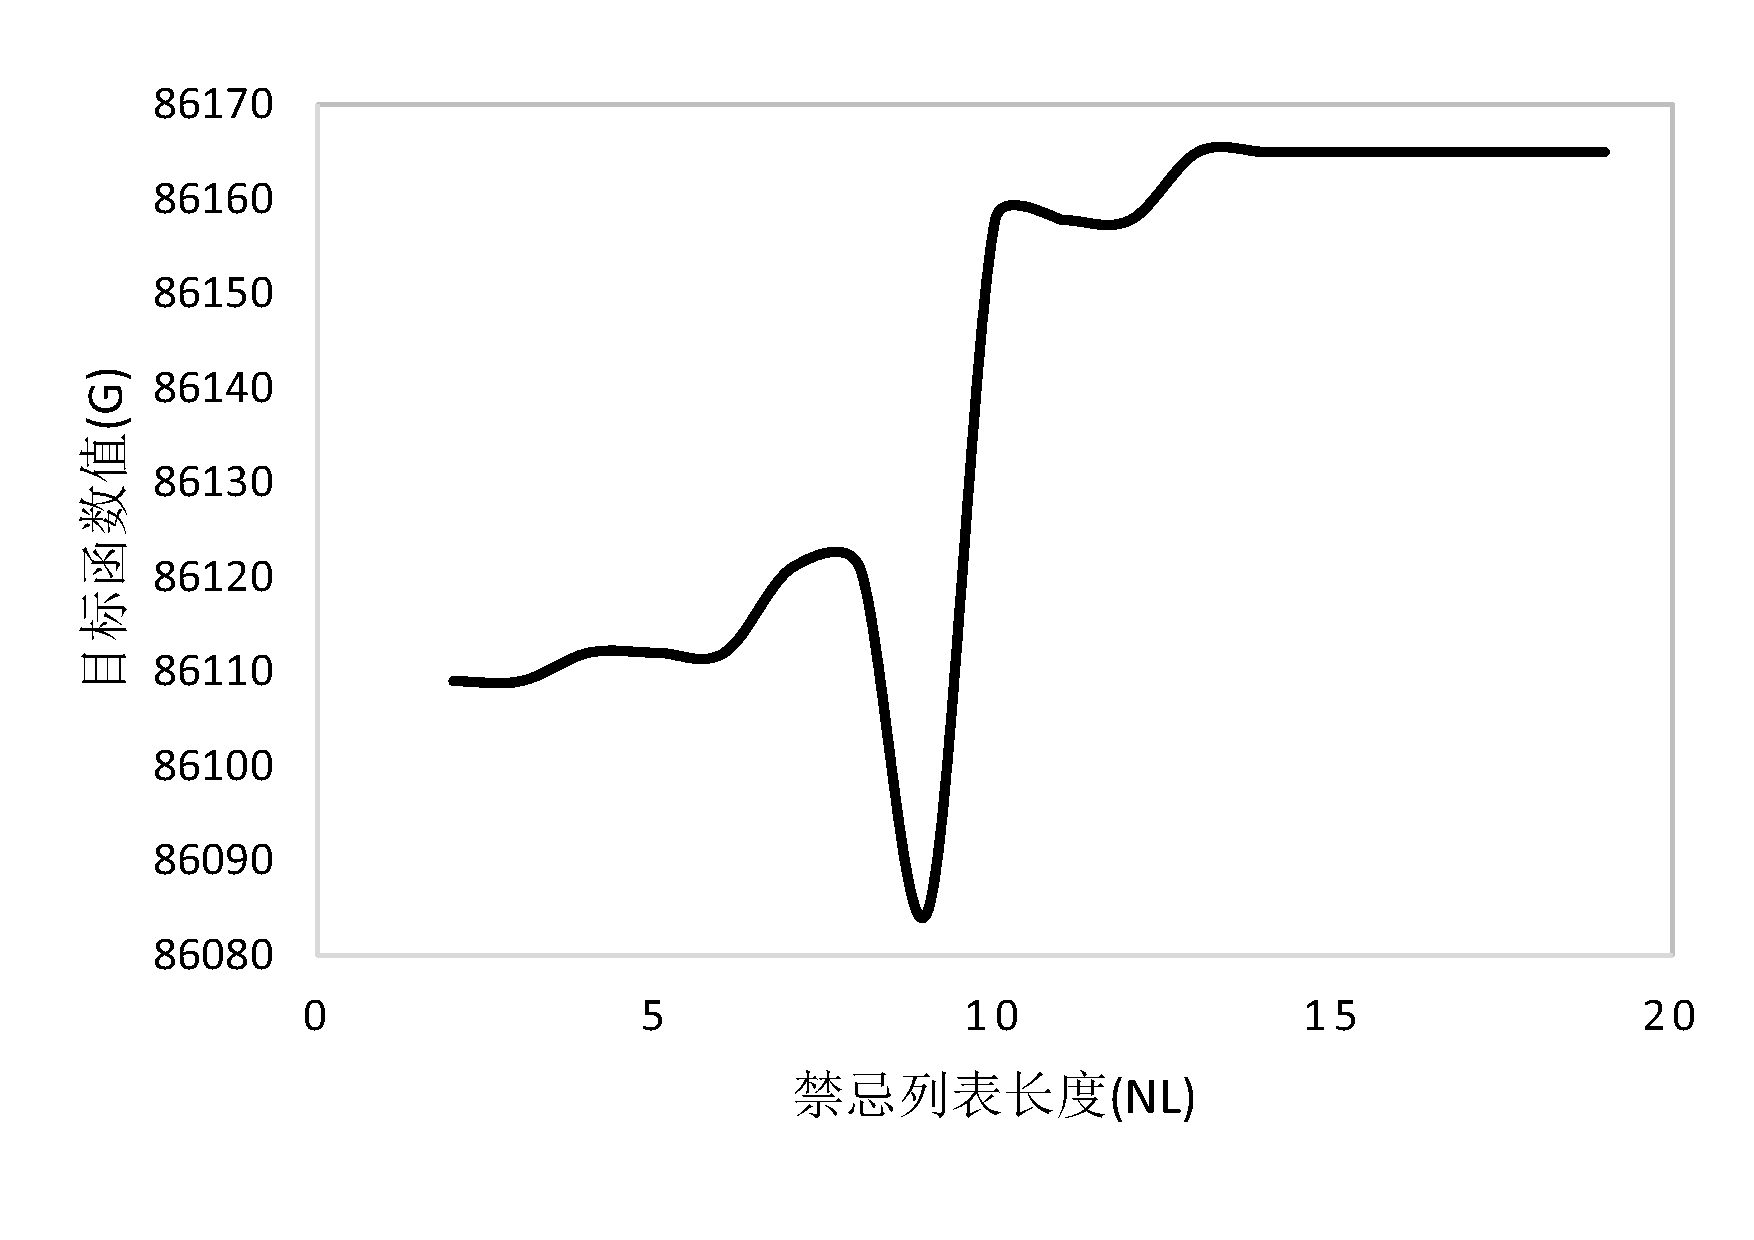
\includegraphics[height= 8.2cm,angle = -90]{NL_100}\label{fig:100NLwithGoal}}
\subfloat[迭代次数]{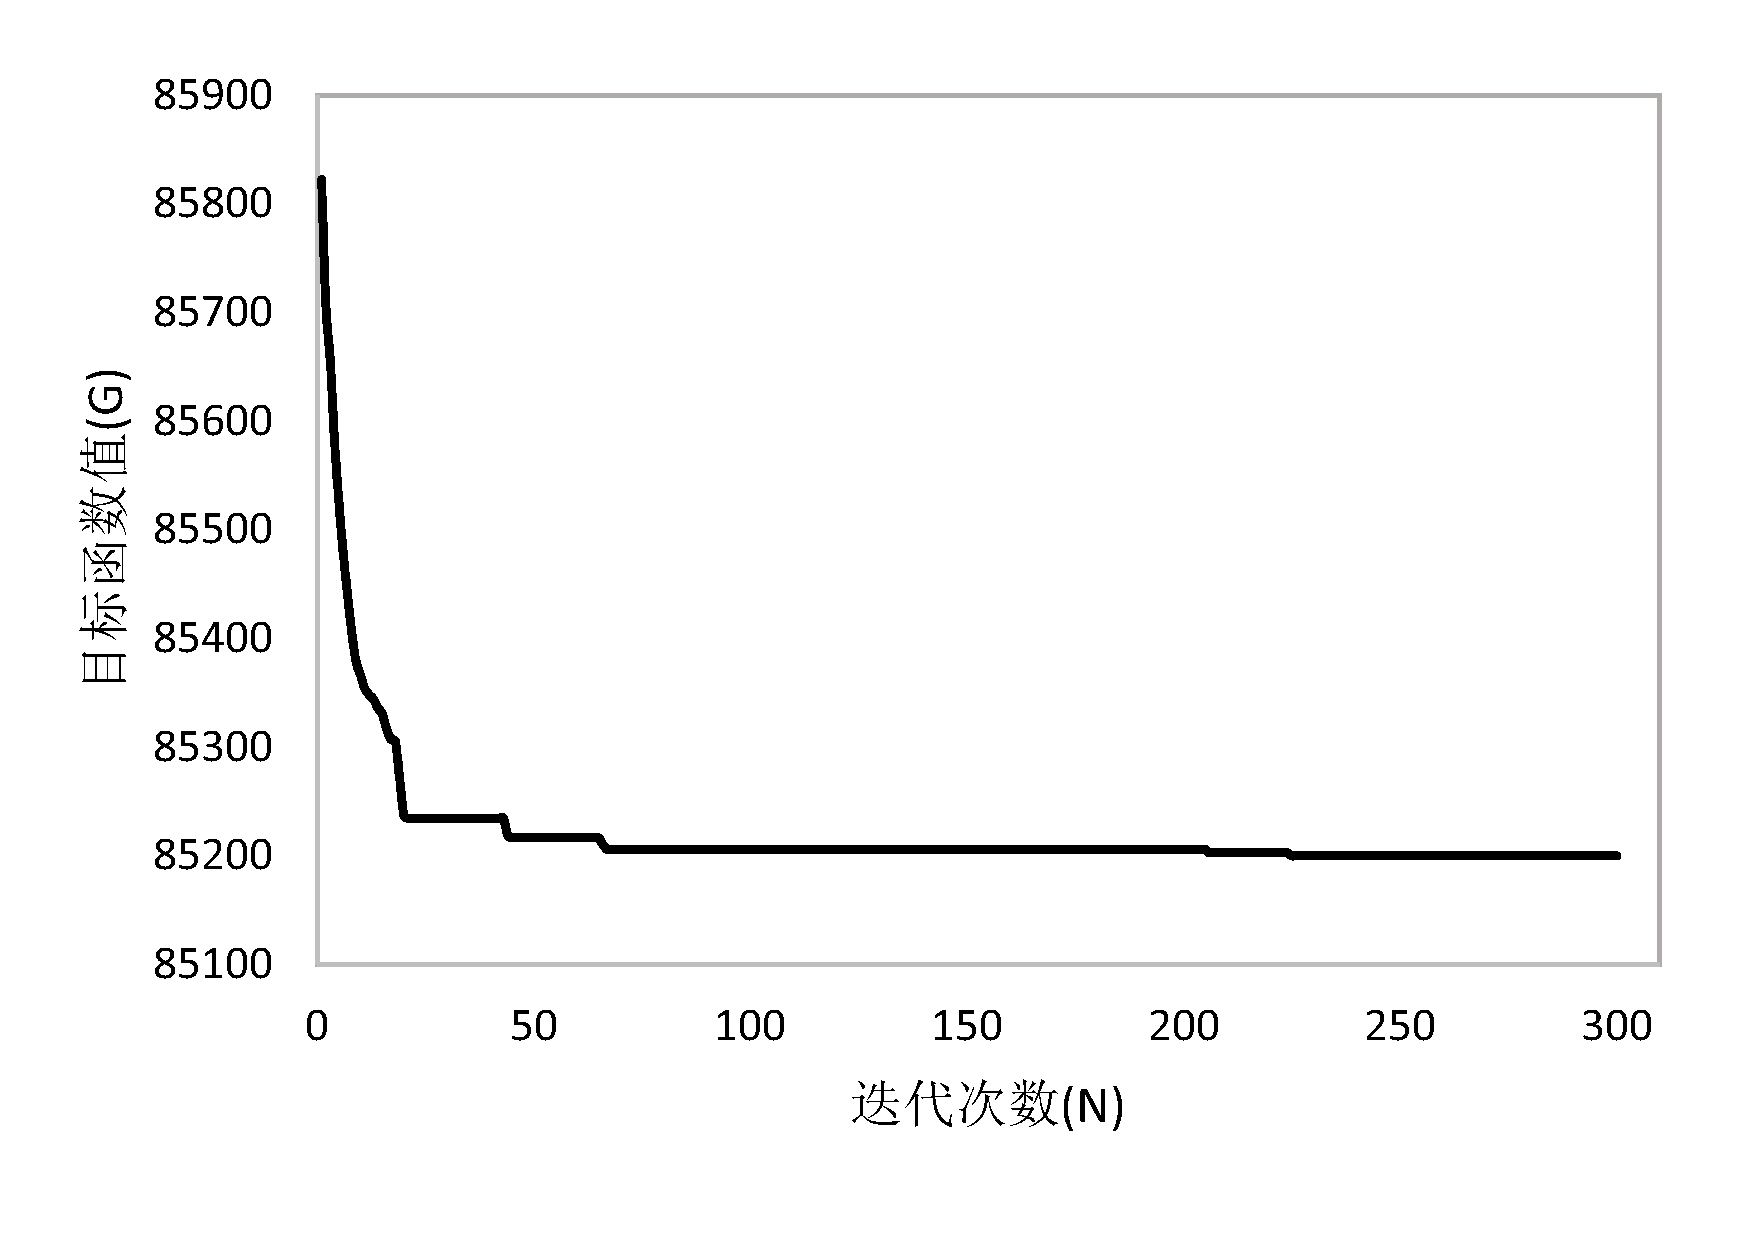
\includegraphics[height= 8.2cm,angle = -90]{N_100}\label{fig:100NwithGoal}}
\caption{$100$件订单的目标函数值和相关参数的关系}
\end{figure}

可以看出$NL = 9$是最佳列表长度,确定该值后,以$50$为间隔\footnote{间隔应视订单数量而定,订单越多,间隔越大},生成目标函数值与迭代次数的关系,如\reff{fig:100NwithGoal}所示。
虽然随着迭代次数的增加,目标函数值仍然会减少,其减少幅度不大,并且运算时间增加很多,所以取迭代次数$N = 500$是较为适宜的\footnote{实际上$\left. G\right|_{N=500} = 84997.2, \left. G\right|_{N=1200} = 84972.8$,两者相差仅$0.0287\%$}。

以此类推,可以确定不同问题规模下的这两个参数的值\footnote{经测试,不用决策环境$(\lambda_1, \lambda_2, \sigma)$下,禁忌列表长度$NL$和迭代次数$N$基本不变,所以这两个参数适用于不同的决策环境下},其结果如所示。
\begin{table}[htbp]
  \centering
  \caption{Add caption}
    \begin{tabular}{cccccccccccccc}
    \toprule
    $m $    & \multicolumn{2}{c}{参数} & 20    & 30    & 50    & 70    & 100   & 150   & 200   & 300   & 500   & 750   & 1000 \\
    \midrule
    \multirow{4}[0]{*}{5} & \multirow{2}[0]{*}{基本模型} & $N$    & 2     & 2     & 8     & 6     & 9     & 13    & 27    & 18    &       &       &  \\
          &       & $NL$    &       &       &       &       &       &       &       &       &       &       &  \\
          & \multirow{2}[0]{*}{插单模型} & $N$    & 2     &       &       &       &       &       &       &       &       &       &  \\
          &       & $NL$    &       &       &       &       &       &       &       &       &       &       &  \\
    \multirow{4}[0]{*}{6} & \multirow{2}[0]{*}{基本模型} & $N$    & 2     &       &       &       &       &       &       &       &       &       &  \\
          &       & $NL$    &       &       &       &       &       &       &       &       &       &       &  \\
          & \multirow{2}[0]{*}{插单模型} & $N$    & 2     &       &       &       &       &       &       &       &       &       &  \\
          &       & $NL$    &       &       &       &       &       &       &       &       &       &       &  \\
    \multirow{4}[0]{*}{7} & \multirow{2}[0]{*}{基本模型} & $N$    & 2     &       &       &       &       &       &       &       &       &       &  \\
          &       & $NL$    &       &       &       &       &       &       &       &       &       &       &  \\
          & \multirow{2}[0]{*}{插单模型} & $N$    & 2     &       &       &       &       &       &       &       &       &       &  \\
          &       & $NL$    &       &       &       &       &       &       &       &       &       &       &  \\
    \bottomrule
    \end{tabular}%
  \label{tab:addlabel}%
\end{table}%


\section{算法评价体系}


\section{参数确定}

\section{结果及评估}

\section{小结}